\documentclass[a4paper, oneside, 12pt]{article}

\usepackage{../custom}

\usepackage[backend=biber]{biblatex}
\addbibresource{../biblio.bib}

\title{Tâche 2}
\author{Groupe 1225}
\date{\today}

\begin{document}

\maketitle

\section{Analyse des conditions optimales du réacteur de synthèse d'ammoniac}

Jusqu'ici nous avons considéré la dernière étape du procédé - la synthèse d'ammoniac -
comme une bo\^ite noire. Nous allons maintenant déterminer quelles sont les conditions 
optimales de température et de pression pour ce réacteur. 
Avant de commencer, il nous semble important de rappeler le principe 
de \textsc{Le Ch\^atelier} : \enquote{Si l'on tend à modifier les conditions d'un système en équilibre, 
il réagit de façon à s'opposer, en partie, aux changements qu'on lui impose, 
jusqu'à l'établissement d'un nouvel équilibre.}. \cite{chatelier}

La réaction de synthèse l'ammoniac est la suivante
\[\ce{N2_{(g)} + 3H2_{(g)} <=> 2NH3_{(g)} } \]

\paragraph{Pression}

On voit tout de suite que le nombre de moles de gaz de réactifs est supérieur 
au nombre de moles de gaz des produits, 
plus précisément $n_{g}\text{(réactifs)} = 2 \cdot n_{g}\text{(produits)}$.

Par la loi des gaz parfait, on sait que la pression est directement proportionnelle 
au nombre de moles de gaz. Le principe énoncé ci-dessus
nous permet de dire qu'une \emph{augmentation} de la pression du réacteur ($p_{\text{total}}$),
favorisera le sens de la diminution du nombre de moles de gazs, 
et dans notre cas, favorisera la production de \ce{NH3}.

\[
K = \frac{p_{eq,\ce{NH3}}^2}{p_{eq,\ce{H2}}^3 \cdot p_{eq,\ce{N2}} \cdot p_{\text{total}}^2}
\]
\paragraph{Température}

La réaction de synthèse est une réaction fortement exothermique 
(à $700\si{\kelvin}$, $\Delta_r H^{\circ} = -52.6\si{\kilo\joule}$).
Pour favoriser la réaction dans le sens de production des produits,
il faut donc faire une \emph{diminution} de la température.

\[
K = \exp{\left( \frac{- \Delta_r H^{\circ} + T \, \Delta_r S^{\circ}}{R T}\right)}
\]

\paragraph{Limite sur la température imposée par le catalyseur}

Après quelques recherches sur internet \cite{catalyseur}, nous avons découvert que les catalyeurs utilisés
pour le production d'ammoniac en mileu industriel contenaient principalement du fer (type \ce{Fe3O4}). 
Pour une usine produisant des quantités de \ce{NH3} similaire à la notre (~1500T/jour), une quantité de 100 tonnes
de catalyseur a une durée de vie d'environ 10 ans. Etant donné que notre la réaction de production de l'ammoniac est
endothermique, on s'attend à ce que la réaction se déplace vers le droite pour une température plus basse et c'est le cas.
Cependant le catalyseur ne se comporte pas de la m\^eme manière à toutes les températures. Et il s'avère que dans notre
cas, le catalyseur n'est pas efficace à basse température. C'est la raison pour laquelle il ne faut pas effectuer
cette reaction à basse température comme le suggerait nos premières observations.

\paragraph{Limite sur la pression imposée par les matériaux du réacteur}

\section{Modélisation par \textsc{Aspen Plus}}
\subsection{Démarrage}

Lors de la première tâche, nous analysions l'installation dans son ensemble, 
mais de manière excessivement simplifiée. 
Dans cette section, nous nous concentrerons sur l'explicitation de la dernière étape 
pour ensuite la simuler sur le logiciel \textsc{Aspen Plus}. 
Nous ne désirons plus la considérer comme une boîte noire, et l'avons donc découpée 
en un certain nombre de processus intermédiaires. 

Le gaz composé d'\ce{N2}, d'\ce{H2} et d'\ce{Ar} passe par un réchauffeur 
et par un compresseur pour atteindre respectivement la température et la pression voulue. 
Il va ensuite dans le réacteur où se déroule la réaction.
Le produit est refroidit dans une installation prévue à cette fin, 
pour arriver enfin dans un séparateur où on extrait l'ammoniac.

Il semblait intéressant de créer un circuit de recyclage pour réutiliser 
le mélange de \ce{N2} et de \ce{H2} issus du processus (la réaction n'est pas complète 
et il reste donc des réactifs). Malheureusement, il y existe également de l'argon 
qu'on ne peut séparer du reste. En effet, sa température d'ébullition est bien trop 
proche de celle des autres composés et les moyens à mettre en œuvre en seraient 
très couteux et/ou à faible rendement.

Notre groupe a donc décidé de faire une purge dans le circuit de recyclage afin d'éviter que l'argon ne s'accumule. Cette purge ne doit pas être trop grande sinon la quantité perdue des réactifs serait conséquente. 
La condition à respecter est donc d'avoir un flux entrant d'argon égal à celui de sortie. 
Les calculs permettant de trouver la quantité parfaite à purger 
sont détaillés dans la sous-section suivante.

Le flowsheet de notre installation correspondant à la modélisation 
du réacteur de synthèse sur \textsc{Aspen Plus} 
se trouve dans la figure \ref{fig:flow_aspen}.
Afin d'apporter plus de précision, nous avons également réalisé un petit 
flowsheet de la même partie du procédé qui détaille le parcours des 
différents réactifs et leurs états à travers le processus.
Le diagramme se trouve dans la figure \ref{fig:flow_synthese}.

\begin{figure}[h!]
	\begin{center}
		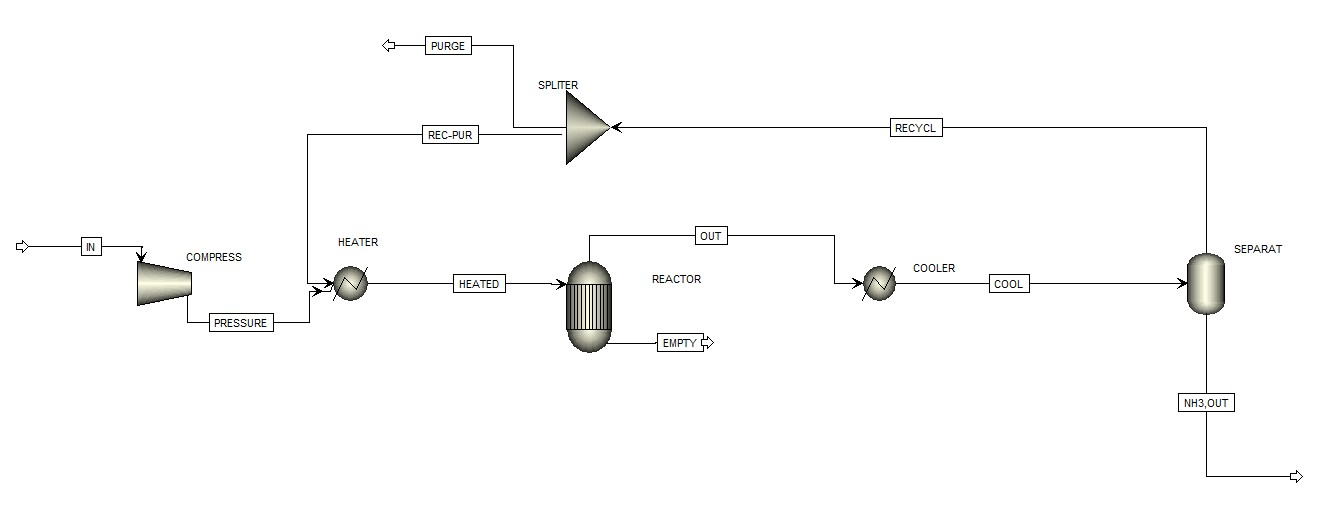
\includegraphics[scale=0.45,angle=90]{img_aspen/flowsheet.jpg}
	\end{center}
	\caption{Flowsheet de la réaction finale sur \textsc{Aspen Plus}.}
	\label{fig:flow_aspen}
\end{figure}

\subsection{La purge}

Dans les calculs qui suivent, nous cherchons $X$ qui n'est autre que 
la fraction du recyclage qui doit être purgée. 
Nous négligeons l'imperfection du séparateur et faisons donc l'hypothèse 
que l'ammoniac sortant est pur, ce qui est bien sur impossible. 
Nous nous référerons au schéma pour ce qu'il en est des notations. 
Rappelons qu'il est aisé de trouver les débits d'entrée des réactifs 
et de sortie de l'ammoniac grâce à notre outil de calcul.

\begin{figure}[h!]
	\begin{center}
		\begin{tikzpicture}
[node distance = 7em]

\tikzstyle{block} = [rectangle, draw, fill=blue!20, 
    text width=7em, text centered, rounded corners, minimum height=3em]
\tikzstyle{block2} = [rectangle, draw, fill=red!60, 
    text width=6em, text centered, minimum height=2em]
\tikzstyle{line} = [draw, -latex']
\tikzstyle{cloud} = [draw, ellipse,fill=red!20, node distance=2cm,
    minimum height=1em]


\node [cloud] (input) {Input};
\node [block, right = 17em of input] (compresseur) {Compresseur\\Synthèse};
\node [block, below = 6em of compresseur] (separation) {Refroidisseur\\Séparation};
\node [block2,left = 15em of separation] (purge) {Purge};
\node [cloud, below = 5em of purge] (residu) {Résidus};
\node [cloud, below = 4em of separation] (output) {Output};

\path [line] (input) -- node[anchor = south] {\ce{N2} \ce{H2} \ce{Ar}}
	(compresseur);
\path [line,dashed] (compresseur) -- node[anchor = west] { \ce{Ar} \ce{NH3_{(g)}} \ce{NH3_{(l)}}} 
	node[anchor = east] {\ce{N2} \ce{H2}} 
	(separation);
\path [line,dashed] (separation) -- node[anchor = north] {\ce{NH3_{(g)}} 
	\ce{H2} \ce{N2} \ce{Ar}} 
	(purge);
\path [line,dashed] (purge) -- node[anchor = east] {\ce{Ar} 
	\ce{N2} \ce{H2} $\quad$}
	node[anchor = west]{$\quad$ \ce{NH3_{(g)}}} 
	(compresseur);
\path [line] (purge) -- node[anchor = east] {\ce{NH3_{(g)}}}
	node[anchor = west] { \ce{N2} \ce{H2} \ce{Ar}}
	(residu);
\path [line] (separation) -- node[anchor = east] {\ce{NH3_{(l)}}} 
	(output);
\end{tikzpicture}


	\end{center}
	\caption{Schéma simplifié de l'étape finale.}
	\label{fig:flow_synthese}
\end{figure}

Comme dit précédemment, une purge optimale doit permettre un débit 
de sortie d'argon égal à celui d'entrée dans le système. 
On peut écrire ça sous la forme:

\begin{equation}
\dot{n}_{\ce{Ar},\text{in}}=\dot{n}_{\ce{Ar},purge}=x_{\ce{Ar},\text{purge}} \dot{n}_{\text{purge}}
\end{equation}

Ceci est donc le bilan total d'argon. 
Il est possible de faire d'autres bilans afin de nous donner d'autres relations utiles.

$\bullet$ Bilan molaire à la purge:
\begin{equation}
\dot{n}_{\text{purge}} = X \cdot \dot{n}_{\text{recyclage}}
\label{eq:bilan_mol_purge}
\end{equation}

$\bullet$ Bilan molaire au séparateur:
\begin{equation}
\dot{n}_{\text{out}}=\dot{n}_{\text{recyclage}}+\dot{n}_{\ce{NH3},\text{out}}
\label{eq:bilan_mol_sep}
\end{equation}

$\bullet$ Bilan d'argon au séparateur:
\begin{equation}
x_{Ar,\text{out}} \dot{n}_{\text{out}}=x_{\ce{Ar},\text{recyclage}} \dot{n}_{\text{recyclage}}
\end{equation}

$\bullet$ Bilan molaire total:

\begin{equation}
	\dot{n}_{in} - 2\xi=\dot{n}_{\ce{NH3},\text{out}} + \dot{n}_{\text{purge}}
	\label{eq:bilan_mol_tot}
\end{equation}

avec $\xi$ étant l'avancement, c'est à dire le nombre de moles de \ce{N2} ayant réagit. 
Faisons attention de noter qu'on ne considère que les réactifs venant du circuit $in$. 
Cela est résumé dans le tableau suivant. 
On analyse le débit de moles à l'entrée du réacteur pour les différents composés, 
ainsi qu'à la sortie (on considère que l'équilibre a été atteint).

\begin{table}[h!]
	\centering
	\begin{tabular}{l|c|c|c|c}
		$\ce{N2}$ & $\ce{H2}$ & $\ce{Ar}$ & $\ce{NH3}$ & $n_{total}$ \\
		\hline
		$n_{\ce{N2},in}$ & $n_{\ce{H2},in}$ & $n_{\ce{Ar},in}$ & $0$  & $n_{in}$\\
		$n_{\ce{N2},in}-\xi$ & $n_{\ce{H2},in}-3\xi$ & $n_{\ce{Ar},in}$ & $2\xi$  & $n_{in}-2\xi$\\
	\end{tabular}
	\caption{Réaction dans le réacteur.}
	\label{tab:reaction1_primaire}
\end{table}

La réaction se déroule à une certaine température T et à une pression p. 
Il est facile de calculer $K$ en trouvant $\Delta_r G$ au préalable. 
Nous pouvons faire cela en utilisant notre outil de calcul.

\[
K=\exp{\left(\frac{-\Delta G}{R \cdot T}\right)}\]

L'expression de la constante d'équilibre $K_p$ est également: 

\[
K_p=\frac{{x_{\ce{NH3},\text{out}}}^2}{x_{\ce{N2},\text{out}}{x_{\ce{H2},\text{out}}}^3} \cdot p^{-2} = 
\frac{{n_{\ce{NH3},\text{out}}}^2}{n_{\ce{N2},out}\cdot {n_{\ce{H2},out}}^3}\cdot {n_{\text{total,out}}}^2\cdot p^{-2}
\]
si on utilise la loi des gaz parfait et plus précisément celle de Dalton. Faisons attention que c'est une hypothèse simplificatrice forte. 
Comme $n_{\ce{H2}}=3\cdot n_{\ce{N2}}$ (éléments en quantité stœchiométrique), 
on a donc 
$K=\frac{{n_{\ce{NH3},\text{out}}}^2}{27{n_{\ce{N2},out}}^4} \cdot
{n_{\text{total,out}}}^2\cdot p^{-2}$. 
En injectant les quantités des composés du tableaux, fonctions de $\xi$, on obtient:

\[ 
K = 
\frac{({2\xi})^2}{27 \cdot ({{n_{\ce{N2,in}}-\xi})^4}} \cdot
({n_{total,in}-2\xi})^2 \cdot p^{-2} 
\]

Nous pouvons par exemple résoudre cela avec \textsc{matlab}. 
Connaissant $\xi$, on trouve $\dot{n}_{\text{purge}}$
grâce à l'équation \ref{eq:bilan_mol_tot}. 
Nous obtenons directement $x_{\ce{Ar},\text{purge}}$ en injectant 
le résultat dans la première équation. 
$x_{\ce{Ar},\text{purge}}$ est égal à $x_{\ce{Ar},\text{recyclage}}$ 
car la purge n'altère par la concentration.

Nous disposons de la quantité d'ammoniac produite (un paramètre) 
et pouvons donc maintenant connaitre la quantité totale de réactifs restants après réaction. 
Rappelons que les quantité utilisées plus haut ne prenaient pas en compte le recyclage. 
Reprenons l'expression de $K$: 

\[ 
K = 
\frac{{n_{\ce{NH3},\text{out}}}^2}{27{n_{\ce{N2},out}}^4} \cdot 
{n_{\text{total,out}}}^2\cdot p^{-2}
\]

Or nous savons que $\dot{n}_{\text{total,out}} = 
4\dot{n}_{\ce{N2},out}+\dot{n}_{\ce{Ar},out}+\dot{n}_{\ce{NH3},out}$ 

où $\dot{n}_{\ce{Ar},out}$ est successivement:

\[\dot{n}_{\ce{Ar},out}=\dot{n}_{\ce{Ar},\text{recyclage}}\]

\[ \dot{n}_{\ce{Ar},out}=x_{\ce{Ar},\text{recyclage}}\dot{n}_{\text{total,recyclage}} \]

\[ 
\dot{n}_{\ce{Ar},out}\underset{(3)} = 
x_{\ce{Ar},\text{recyclage}}(\dot{n}_{\text{total,out}}-\dot{n}_{\ce{NH3},\text{out}}) 
\]

Nous avons donc 2 équations pour trouver 
les 2 inconnues $n_{\ce{N2},out}$ et $n_{\text{total,out}}$. 
Nous pouvons à nouveau résoudre cela par \textsc{matlab}. 
A présent, il suffit d'utiliser l'équation \ref{eq:bilan_mol_sep} 
pour trouver $\dot{n}_{\text{recyclage}}$. 
Comme nous le dit l'équation \ref{eq:bilan_mol_purge}, 
le rapport de $\dot{n}_{\text{purge}}$ 
et de $\dot{n}_{\text{recyclage}}$ nous donne enfin $X$! 
Ces calculs fastidieux nous permettent donc enfin de trouver la fraction à prélever 
dans le circuit de recyclage. 
Le même cheminement est suivi dans le programme \texttt{purge} 
disponible dans notre outil de gestion. Nous verrons plus loin que ces calculs donnent
des résultats assez loin de la réalité. La fraction minimale a purger est toujours
bien moindre. Cela est du au grand nombre d'hypothèses simplificatrices utilisées. 
La loi des gaz parfaits donne par exemple des résultats très peu précis 
dans de telles conditions de température et de pression. 
De plus, dans des conditions réelles, une séparation parfaite est impossible 
et une partie du \ce{NH3} part avec l'\ce{Ar}.
Cependant, le programme nous donne le type de fonction que la fraction minimale de purge
suit lorsque l'on modifie les paramètres: elle augmente peu avec la pression et diminue
de manière plus conséquente avec la température. Nous pouvons voir cela dans les figures
\ref{fig:purge1} et \ref{fig:purge2}.

\begin{figure}[h!]
	\begin{center}
		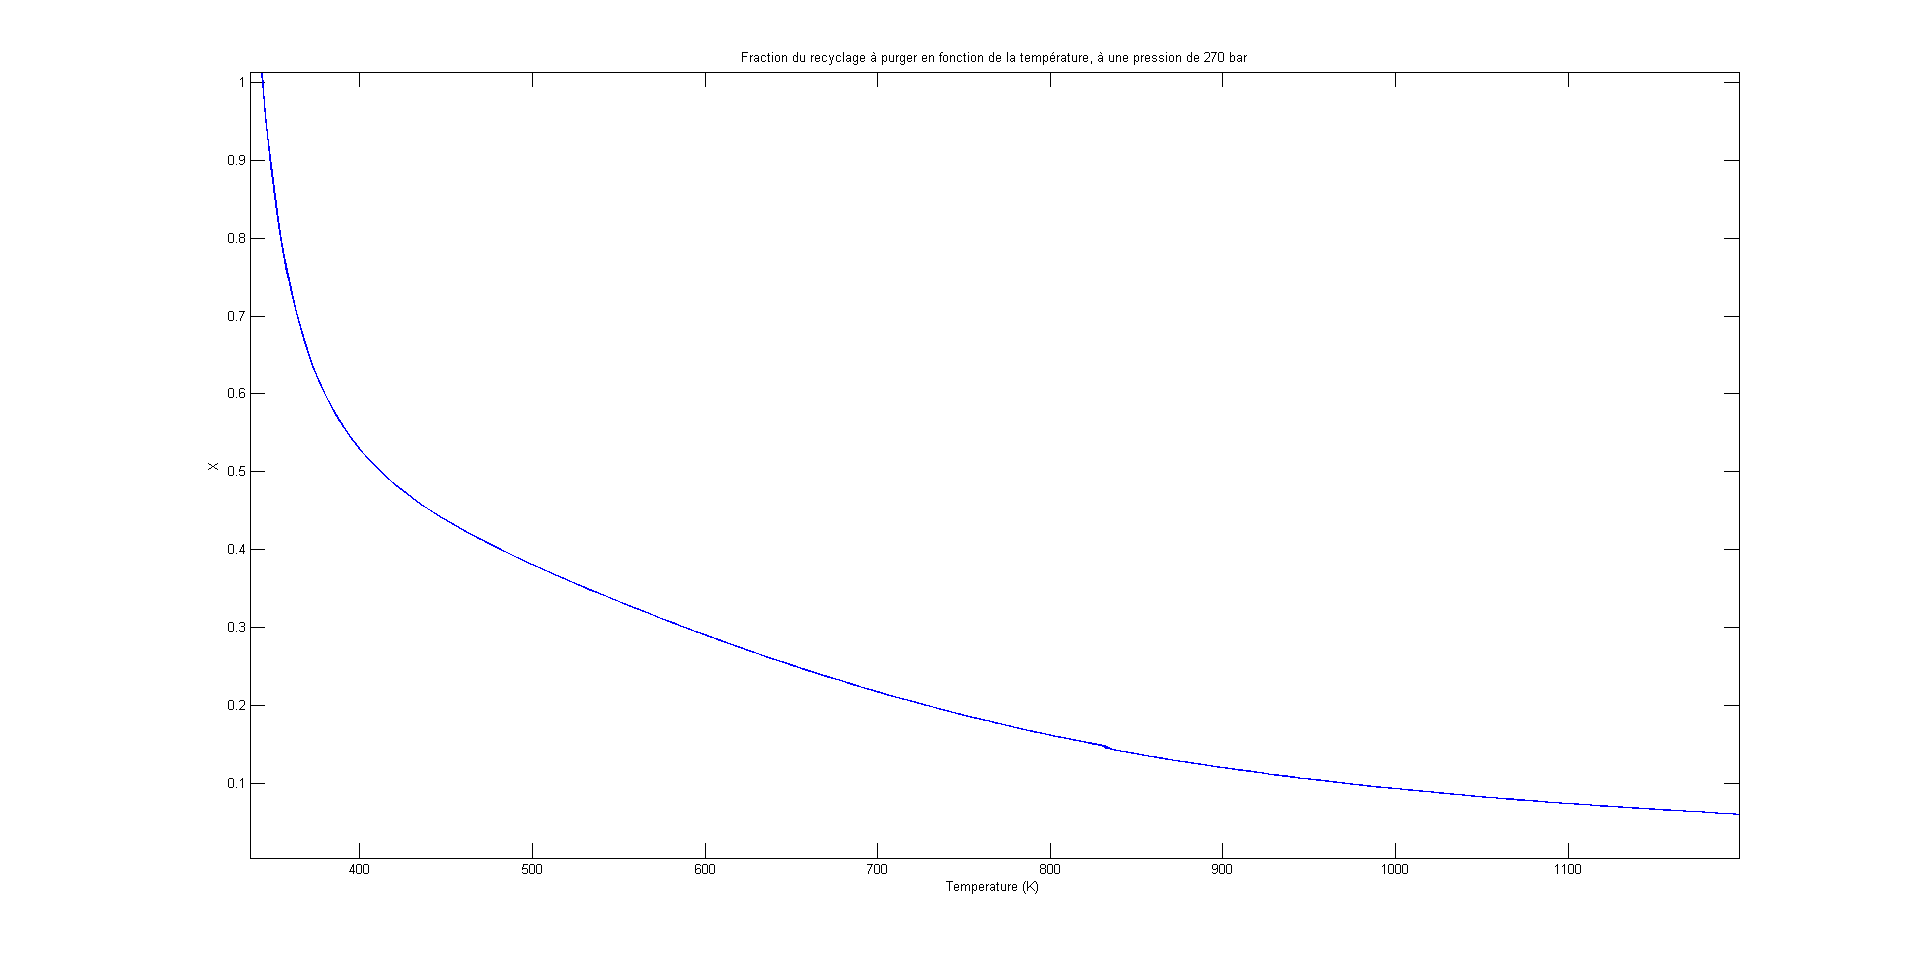
\includegraphics[scale=0.3]{purge1.png}
	\end{center}
	\caption{Fraction de purge en fonction de la température.}
	\label{fig:purge1}
\end{figure}

\begin{figure}[h!]
	\begin{center}
		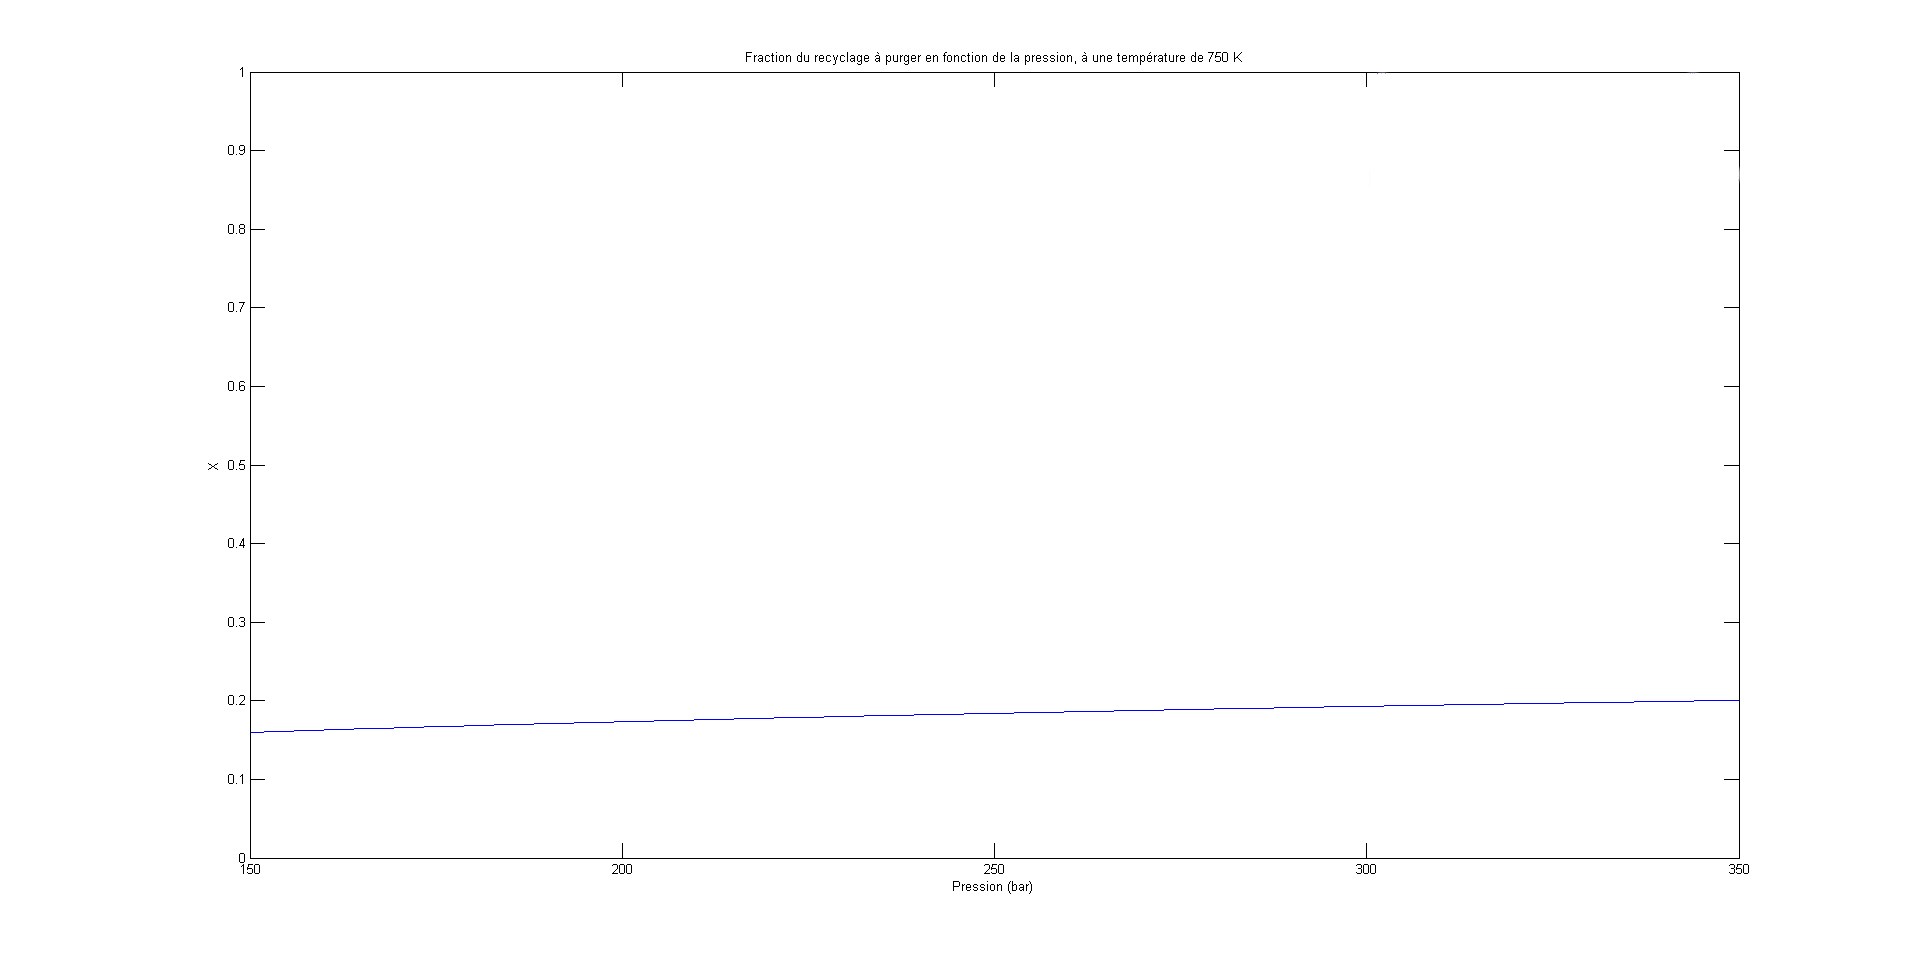
\includegraphics[scale=0.3]{purge2.png}
	\end{center}
	\caption{Fraction de purge en fonction de la pression.}
	\label{fig:purge1}
\end{figure}


\subsection{Validation du modèle}

Le logiciel \textsc{Aspen Plus} propose de nombreuses 
modélisations du comportement des fluides, 
plus ou moins fidèles selon les composés et 
les conditions dans lesquels on les observe. 
Notre recherche s'est limitée aux modèles à haute pression. 

Après en avoir fait l'étude en comparant les bases de données de chacun d'eux, 
nous avons gardé 3 candidats: \texttt{RK-Aspen}, \texttt{PSRK} et \texttt{SRK}. 
Tous trois basés sur les équations de Soave-Redlich-Kwong, 
ils modélisent correctement les gaz légers et non polaires 
comme ceux auxquels nous avons affaire ici. 
Ces modèles sont également les seuls à être capables de faire 
des prédictions correctes à une pression supérieure à $150\si{\bar}$. 
Nous avons donc effectué quelques tests sur chacun des trois 
et nous avons obtenus des résultats assez similaires.
Cependant, le modèle SRK promet de garder sa précision dans des conditions 
quasi critiques, ce qui n'est pas le cas des deux autres. 
La pression dans notre circuit pouvant avoisiner les $270\si{\bar}$, 
c'est ce dernier que nous avons donc choisi pour faire des simulations approfondies.\\
Lors de nos tests, nous avons arbitrairement fixé la température et 
la pression des réactifs entrants respectivement à $25\si{\degreeCelsius}$ et $1\si{\bar}$.

En effet, leurs valeurs exactes nous sont inconnues et n'ont de toute manière 
aucun impact sur le fonctionnement du circuit, grâce à la présence des échangeurs de chaleur 
et du compresseur.

Tout d'abord, nous avons fixé les conditions dans le réacteur à $270\si{\bar}$ 
et $750\si{\kelvin}$. 
Nous avons également choisi de mettre un certain flux de \ce{H2}, \ce{N2}, et d' \ce{Ar} 
pour lesquels nous connaissions le flux théorique correspondant de \ce{NH3} à la sortie,
grâce au tableau de données reçu à la tâche~1. 
Nous avons également fixé le pourcentage du recyclage à purger à $5\%$ pour nos tests.\\

Pour les conditions décrites ci-dessus, 
nous avons obtenu après simulation un flux de \ce{NH3} légèrement inférieur à nos attentes. 
Cela s'explique à nouveau par le fait que pour les résultats attendus, 
nous avions négligé les pertes au niveau du séparateur et considéré la réaction complète.
Par la suite, nous avons essayé de faire varier certains paramètres afin 
de voir si les résultats obtenus étaient en adéquation avec nos prédictions. 
Nous avons commencé par diminuer la température et comme nous l'avions prédit, 
la quantité produite d'ammoniac a augmentée. 
Un test avec une température supérieure à $750\si{\kelvin}$ nous a confirmé cela. 
Nous avons ensuite vérifié que nos attentes concernant la pression étaient respectées. 
Et en effet, lorsque nous avons augmenté la pression, 
la quantité produite de \ce{NH3} a faiblement augmenté.

Pour finir, nous avons fait varier les valeurs du pourcentage de la purge.
Il s'est avéré que notre simulation ne convergeait pas en dessous de $4\%$ 
et nous avions des erreurs.
Nous avons ensuite augmenté le pourcentage 
et observé une diminution de la production de \ce{NH3}. 
Ces résultats sont logiques puisque l'augmentation du pourcentage 
de purge est évidemment la cause de pertes de matières premières. 
La quantité de produits en est donc altérée.

Tous les résultats obtenus lors de nos simulations 
sont disponibles dans l'annexe~\ref{sec:aspen_simulation}.

\subsection{Simulation itérative sur \textsc{Matlab}}

Nous pouvions maintenant comparer les résultats
avec ceux de notre propre simulation réalisée sur
textsc{Matlab}. Son fonctionnement est simple:
elle calcule - pour une série d'itérations - 
les différents flux à la sortie du réacteur 
et dans le recyclage grâce à l'avancement de
la réaction. On utilise ensuite ces informations 
de manière récursive pour connaître le débit de 
réactifs entrants au prochain pas de temps. Si 
la différence entre le flux d'argon actuel et 
de l'itération précédente passe en dessous d'un 
certain seuil, on considère que le système s'est 
stabilisé: il a convergé.

Malgré l'imprécision de notre modèle (utilisation
de la loi des gaz parfaits) et la simplification
de l'installation, nos résultats sont 
remarquablement proches de ceux obtenus. Il n'y
a qu'une divergence marquée lorsque l'on travaille 
avec une haute température. A titre d'illustration, 
la figure \ref{tab:sim} nous donne la comparaison 
de résultats venant des deux simulations:

\begin{table}[h!]
	\centering
	\begin{tabular}{l|c|c}
		Paramètres choisis & \textsc{Aspen} & \textsc{Matlab}\\
		\hline
		$m_{\ce{NH3}, parfait}$=1500t/jour, & $n_{\ce{NH3}}$=942,94mol/s, & $n_{\ce{NH3}}$=937,795mol/s,\\
		T=750K, p=270bar, x=5\%             &   &  \\
		\hline
		$m_{\ce{NH3}, parfait}$=1500t/jour, & $n_{\ce{NH3}}$=1011,06mol/s, & $n_{\ce{NH3}}$=999,335mol/s,\\
		T=500K, p=270bar, x=5\%             &   &  \\
		\hline
		$m_{\ce{NH3}, parfait}$=1500t/jour, & $n_{\ce{NH3}}$=929,115mol/s, & $n_{\ce{NH3}}$=931,36mol/s,\\
		T=750K, p=220bar, x=5\%             &   &  \\
		\hline
		$m_{\ce{NH3}, parfait}$=1500t/jour, & $n_{\ce{NH3}}$=883,132mol/s, & $n_{\ce{NH3}}$=869,733mol/s,\\
		T=750K, p=270bar, x=10\%             &   &  \\
		\hline

	\end{tabular}
	\caption{Comparaison des simulations}
	\label{tab:sim}
\end{table}

\appendix
\section{Résultats des simulations sur \textsc{Aspen Plus}}
\label{sec:aspen_simulation}

Nous regroupons dans les figures~\ref{fig:RK-ASPEN} à~\ref{fig:SRK,750,270,1}
tous les résultats produits par nos simulations réalisées sur \textsc{Aspen Plus}. 
Pour chacune d'elles, nous précisons le modèle utilisé,
les conditions de température et de pression dans le réacteur 
et la fraction purgée du recyclage. 
On accorde en particulier de l'attention aux résultats 
concernant les deux flux suivants: \textsc{nh3,out} et \textsc{purge}.

\graphicspath{{./img_aspen/}}

\begin{figure}[h!]
	\begin{center}
		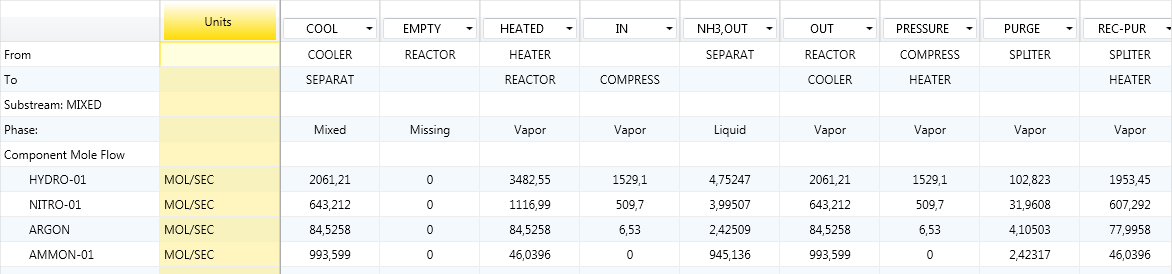
\includegraphics[scale=0.5]{RK-ASPEN.png}
	\end{center}
	\caption{Modèle \texttt{RK-ASPEN}, $750\si{\kelvin}$, $270\si{\bar}$, 5\%}
	\label{fig:RK-ASPEN}
\end{figure}

\begin{figure}[h!]
	\begin{center}
		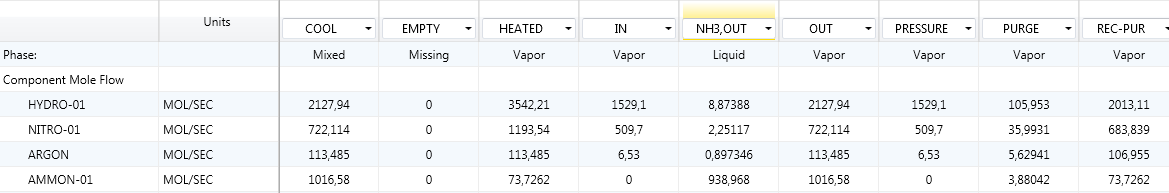
\includegraphics[scale=0.5]{PSRK.png}
	\end{center}
	\caption{Modèle \texttt{PSRK}, $750\si{\kelvin}$, $270\si{\bar}$, 5\%}
	\label{fig:PSRK}
\end{figure}

\begin{figure}[h!]
	\begin{center}
		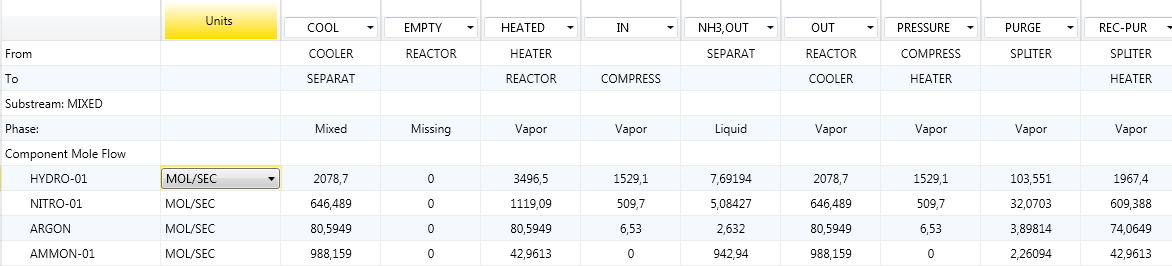
\includegraphics[scale=0.5]{SRK,750,270,5.png}
	\end{center}
	\caption{Modèle \texttt{SRK}, $750\si{\kelvin}$, $270\si{\bar}$, 5\%}
	\label{fig:SRK,750,270,0.05}
\end{figure}

\begin{figure}[h!]
	\begin{center}
		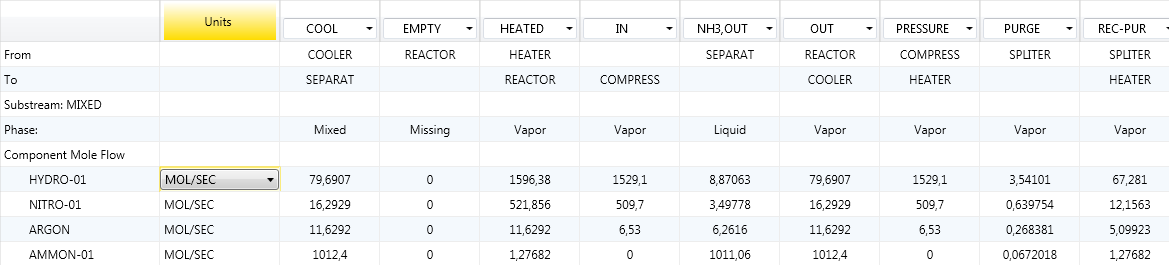
\includegraphics[scale=0.5]{SRK,500,270.png}
	\end{center}
	\caption{Modèle \texttt{SRK}, $500\si{\kelvin}$, $270\si{\bar}$, 5\%}
	\label{fig:SRK,500,270,0.05}
\end{figure}

\begin{figure}[h!]
	\begin{center}
		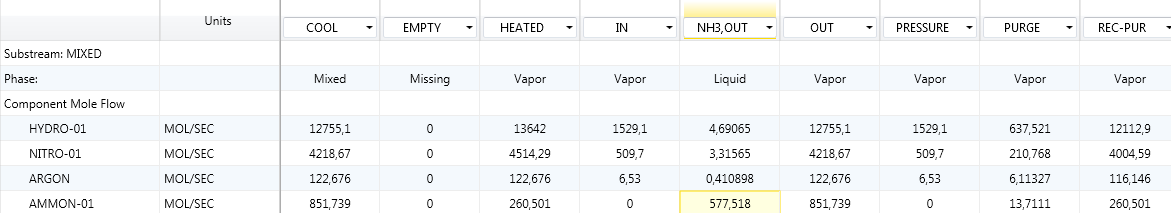
\includegraphics[scale=0.5]{SRK,1000,270.png}
	\end{center}
	\caption{Modèle \texttt{SRK}, $1000\si{\kelvin}$, $270\si{\bar}$, 5\%}
	\label{fig:SRK,1000,270,0.05}
\end{figure}

\begin{figure}[h!]
	\begin{center}
		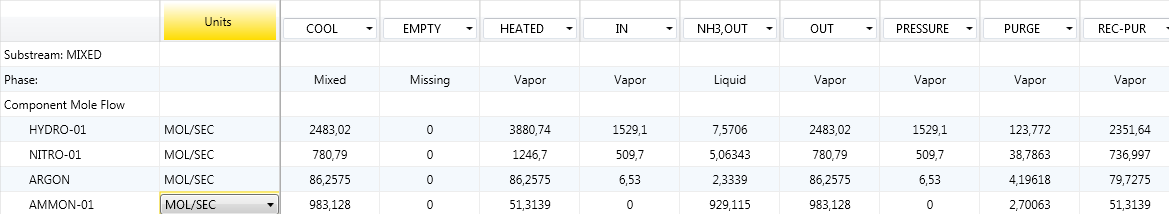
\includegraphics[scale=0.5]{SRK,750,220.png}
	\end{center}
	\caption{Modèle \texttt{SRK}, $750\si{\kelvin}$, $220\si{\bar}$, 5\%}
	\label{fig:SRK,750,220,0.05}
\end{figure}

\begin{figure}[h!]
	\begin{center}
		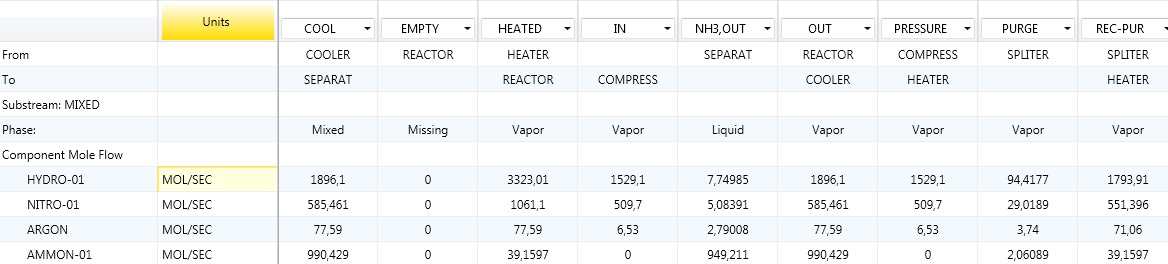
\includegraphics[scale=0.5]{SRK,750,300.png}
	\end{center}
	\caption{Modèle \texttt{SRK}, $750\si{\kelvin}$, $300\si{\bar}$, 5\%}
	\label{fig:SRK,750,300,0.05}
\end{figure}

\begin{figure}[h!]
	\begin{center}
		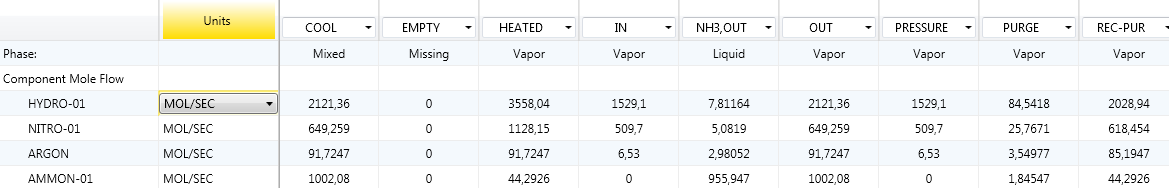
\includegraphics[scale=0.5]{SRK,750,270,4.png}
	\end{center}
	\caption{Modèle \texttt{SRK}, $750\si{\kelvin}$, $270\si{\bar}$, 4\%}
	\label{fig:SRK,750,270,0.04}
\end{figure}

\begin{figure}[h!]
	\begin{center}
		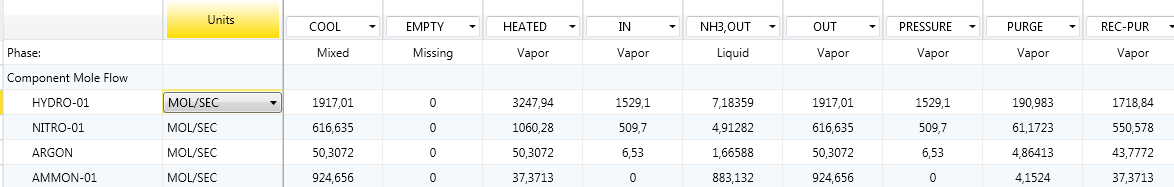
\includegraphics[scale=0.5]{SRK,750,270,10.png}
	\end{center}
	\caption{Modèle \texttt{SRK}, $750\si{\kelvin}$, $270\si{\bar}$, 10\%}
	\label{fig:SRK,750,270,0.1}
\end{figure}

\begin{figure}[h!]
	\begin{center}
		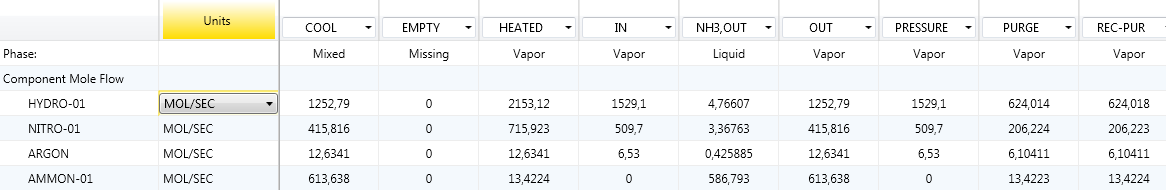
\includegraphics[scale=0.5]{SRK,750,270,50.png}
	\end{center}
	\caption{Modèle \texttt{SRK}, $750\si{\kelvin}$, $270\si{\bar}$, 50\%}
	\label{fig:SRK,750,270,0.5}
\end{figure}

\begin{figure}[h!]
	\begin{center}
		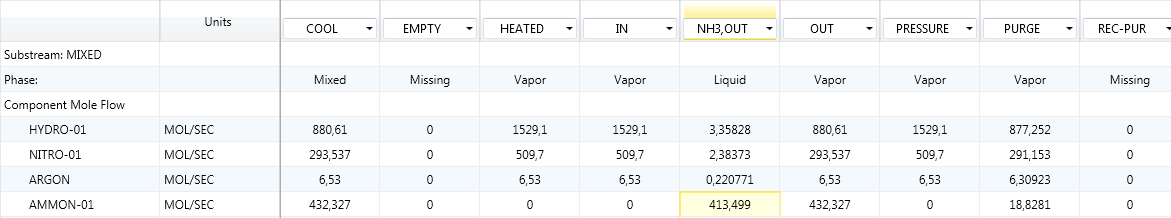
\includegraphics[scale=0.5]{SRK,750,270,100.png}
	\end{center}
	\caption{Modèle \texttt{SRK}, $750\si{\kelvin}$, $270\si{\bar}$, 100\%}
	\label{fig:SRK,750,270,1}
\end{figure}

\section{Outil de calcul: codes \textsc{Matlab}}




\printbibliography
\end{document}

